% nyenje_presentation_final.tex
\documentclass[10pt]{beamer}
\usetheme{Madrid}
\usecolortheme{beaver}
\usepackage[utf8]{inputenc}
\usepackage{amsmath}
\usepackage{amsfonts}
\usepackage{graphicx}
\usepackage{booktabs}
\usepackage{array}
\usepackage{xcolor}
\usepackage{tikz}
\usetikzlibrary{shapes,arrows,positioning}

% Define colors
\definecolor{primary}{RGB}{30,60,114}
\definecolor{secondary}{RGB}{42,82,152}
\definecolor{success}{RGB}{40,167,69}
\definecolor{info}{RGB}{23,162,184}
\definecolor{warning}{RGB}{255,193,7}

% Beamer settings
\setbeamercolor{title}{fg=white,bg=primary}
\setbeamercolor{frametitle}{fg=primary}
\setbeamercolor{block title}{fg=white,bg=secondary}
\setbeamercolor{block body}{bg=gray!10}

% Title information
\title{Nyenje Bay Wind/Waves Analysis Tool}
\subtitle{Technical Presentation and Validation Results}
\author{Key Informatics}
\institute{Lake Kariba, Zambia / Zimbabwe}
\date{April 2026}

\begin{document}

% ============================================================================
% TITLE SLIDE
% ============================================================================
\begin{frame}
\titlepage
\end{frame}

% ============================================================================
% OUTLINE
% ============================================================================
\begin{frame}{Presentation Outline}
\tableofcontents
\end{frame}

% ============================================================================
% SECTION 1: INTRODUCTION
% ============================================================================
\section{Introduction}

\begin{frame}{Project Overview}
\begin{columns}
\column{0.5\textwidth}
\begin{block}{Location}
Nyenje Bay, Lake Kariba\\
\alert{16.53S, 28.83E}
\end{block}

\begin{block}{Objective}
Characterize wind and wave climate for\\
\textbf{Floating Photovoltaic (FPV)} design
\end{block}

\column{0.5\textwidth}
\begin{block}{Data Sources}
\begin{itemize}
    \item ERA5 reanalysis (1971-2020)
    \item CCMP satellite (debiasing)
    \item Kariba Airport (validation)
    \item Local bathymetry survey
\end{itemize}
\end{block}
\end{columns}
\end{frame}

\begin{frame}{Tool Architecture}
\begin{center}
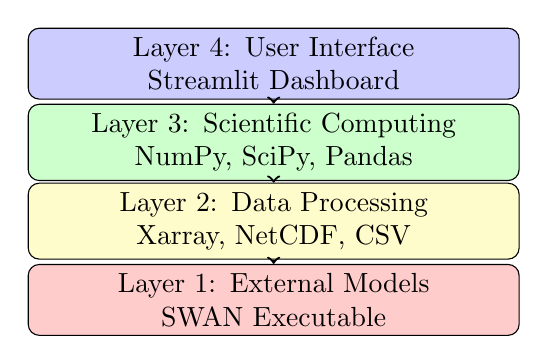
\begin{tikzpicture}[node distance=1cm, scale=0.7]
    \node[draw, fill=blue!20, rounded corners, text width=6cm, text centered] (ui) {Layer 4: User Interface\\Streamlit Dashboard};
    \node[draw, fill=green!20, rounded corners, text width=6cm, text centered, below of=ui] (sci) {Layer 3: Scientific Computing\\NumPy, SciPy, Pandas};
    \node[draw, fill=yellow!20, rounded corners, text width=6cm, text centered, below of=sci] (data) {Layer 2: Data Processing\\Xarray, NetCDF, CSV};
    \node[draw, fill=red!20, rounded corners, text width=6cm, text centered, below of=data] (swan) {Layer 1: External Models\\SWAN Executable};
    
    \draw[->, thick] (ui) -- (sci);
    \draw[->, thick] (sci) -- (data);
    \draw[->, thick] (data) -- (swan);
\end{tikzpicture}
\end{center}
\end{frame}

% ============================================================================
% SECTION 2: DOMAIN
% ============================================================================
\section{Domain Description}

\begin{frame}{Nyenje Bay Domain}
\begin{columns}
\column{0.5\textwidth}
\begin{block}{Domain Parameters}
\begin{tabular}{lc}
\hline
\textbf{Parameter} & \textbf{Value} \\
\hline
Width & 4000 m \\
Height & 3500 m \\
Grid X & 9 points \\
Grid Y & 8 points \\
Total Points & 72 \\
Spacing & 500 m \\
\hline
\end{tabular}
\end{block}

\column{0.5\textwidth}
\begin{block}{Coordinates}
\begin{tabular}{lc}
\hline
\textbf{Boundary} & \textbf{Value} \\
\hline
Center & 16.53S, 28.83E \\
West & 28.81113E \\
East & 28.84887E \\
South & 16.54577S \\
North & 16.51423S \\
\hline
\end{tabular}
\end{block}
\end{columns}
\end{frame}

\begin{frame}{Bathymetry Map (CONSTANT)}
\begin{center}
\fbox{\begin{minipage}{0.8\textwidth}
\centering
\textbf{[Bathymetry Heatmap]}\\
Colors: Viridis (dark blue equals deep, yellow equals shallow)\\
Depth range: 1.2 m to 29.0 m\\
Mean depth: 14.8 m
\end{minipage}}
\end{center}

\begin{itemize}
    \item \textbf{CONSTANT} - Same for all SWAN runs
    \item 9 x 8 grid (72 points)
    \item Deeper in north (up to 29 m), shallower in south (1.2 m)
\end{itemize}
\end{frame}

% ============================================================================
% SECTION 3: WIND ANALYSIS
% ============================================================================
\section{Wind Analysis}

\begin{frame}{Wind Statistics Results}
\begin{columns}
\column{0.5\textwidth}
\begin{block}{Key Statistics}
\begin{tabular}{lc}
\hline
\textbf{Parameter} & \textbf{Value} \\
\hline
Mean Wind Speed & 2.40 m/s \\
Median Wind Speed & 2.21 m/s \\
Maximum Wind Speed & \alert{8.90 m/s} \\
Year of Maximum & \alert{1996} \\
Mean Direction & 51.6 degrees \\
Prevailing Direction & \textbf{NE} \\
\hline
\end{tabular}
\end{block}

\column{0.5\textwidth}
\begin{block}{Interpretation}
\begin{itemize}
    \item Very calm conditions
    \item Fetch-limited bay
    \item Ideal for FPV
\end{itemize}
\end{block}
\end{columns}
\end{frame}

\begin{frame}{Wind Averaging Periods}
\begin{table}
\centering
\begin{tabular}{lcc}
\hline
\textbf{Period} & \textbf{Gust Factor} & \textbf{Calculated} \\
\hline
Hourly Mean & 1.00 & 8.90 m/s \\
3-Minute Average & 1.15 & 10.24 m/s \\
10-Minute Average & 1.00 & 8.90 m/s \\
\alert{3-Second Gust} & \alert{1.45} & \alert{12.91 m/s} \\
10-Second Gust & 1.35 & 12.02 m/s \\
\hline
\end{tabular}
\end{table}

\begin{example}
For maximum wind of 8.90 m/s:
\begin{itemize}
    \item 3-second gust = \alert{12.91 m/s} (ULS design)
    \item 10-second gust = 12.02 m/s (SLS design)
\end{itemize}
\end{example}
\end{frame}

\begin{frame}{EWMA Formula for Wind Averaging}
\begin{block}{Exponential Weighted Moving Average}
\[
\mbox{EWMA}_t = \alpha \cdot x_t + (1 - \alpha) \cdot \mbox{EWMA}_{t-1}
\]
\[
\alpha = \frac{2}{\mbox{span} + 1}
\]
\end{block}

\begin{block}{Parameters}
\begin{itemize}
    \item 3-minute average: span = 3, $\alpha = 0.5$
    \item 10-minute average: span = 10, $\alpha = 0.18$
\end{itemize}
\end{block}
\end{frame}

% ============================================================================
% SECTION 4: WAVE ANALYSIS
% ============================================================================
\section{Wave Analysis}

\begin{frame}{JONSWAP Wave Formula}
\begin{block}{Dimensionless Fetch}
\[
\tilde{x} = \frac{g \cdot F}{U^2}
\]
\end{block}

\begin{block}{Significant Wave Height}
\[
H_s = 0.0016 \cdot \frac{U^2}{g} \cdot \sqrt{\tilde{x}}
\]
\end{block}

\begin{block}{Peak Wave Period}
\[
T_p = 0.286 \cdot \frac{U}{g} \cdot (\tilde{x})^{0.33}
\]
\end{block}

\begin{example}
For U = 8.90 m/s, F = 4 km:
\[
H_s = 0.206 \mbox{ m (20.6 cm)}
\]
\end{example}
\end{frame}

\begin{frame}{Wave Statistics Results}
\begin{table}
\centering
\begin{tabular}{lc}
\hline
\textbf{Parameter} & \textbf{Value} \\
\hline
Yearly Maximum Wave Height & 0.206 m \\
Mean Wave Height & 0.15 m \\
\hline
\end{tabular}
\end{table}

\begin{center}
\color{success}{\Large All waves less than 25 cm!}
\end{center}

\begin{itemize}
    \item Extremely calm wave conditions
    \item Fetch-limited (max 4 km)
    \item Natural wave attenuation
\end{itemize}
\end{frame}

\begin{frame}{Extreme Value Analysis - Return Periods}
\begin{table}
\centering
\begin{tabular}{lcc}
\hline
\textbf{Return Period} & \textbf{Wind (m/s)} & \textbf{Wave (m)} \\
\hline
2-year & 11.2 & 0.174 \\
5-year & 12.8 & 0.188 \\
10-year & 14.0 & 0.197 \\
25-year & 15.6 & 0.208 \\
\alert{50-year} & \alert{16.8} & \alert{0.217} \\
\alert{100-year} & \alert{18.0} & \alert{0.225} \\
\hline
\end{tabular}
\end{table}

\begin{block}{Gumbel Distribution}
\[
x(T) = \mu - \beta \cdot \ln\left(-\ln\left(1 - \frac{1}{T}\right)\right)
\]
\end{block}
\end{frame}

% ============================================================================
% SECTION 5: SWAN MODEL
% ============================================================================
\section{SWAN Model}

\begin{frame}{SWAN Wave Distribution}
\begin{center}
\fbox{\begin{minipage}{0.7\textwidth}
\centering
\textbf{[Wave Height Distribution Map]}\\
9x8 grid showing wave heights in cm\\
Colors: RdYlGn (red equals high, green equals low)
\end{minipage}}
\end{center}

\begin{itemize}
    \item Wave heights vary across domain
    \item Maximum at northeast quadrant
    \item Minimum at southwest (sheltered)
\end{itemize}
\end{frame}

\begin{frame}{SWAN Model Inputs}
\begin{block}{CONSTANT Input}
\textbf{Bathymetry:} Same for all runs
\begin{itemize}
    \item 9x8 grid from survey data
    \item Depth range: 1.2 - 29.0 m
\end{itemize}
\end{block}

\begin{block}{VARIABLE Input}
\textbf{Wind:} Changes each hour
\begin{itemize}
    \item From debiased ERA5 data
    \item u and v components at 72 points
    \item 438,000 total files (1971-2020)
\end{itemize}
\end{block}
\end{frame}

% ============================================================================
% SECTION 6: VALIDATION
% ============================================================================
\section{Validation Results}

\begin{frame}{Validation with Kariba Airport}
\begin{columns}
\column{0.5\textwidth}
\begin{block}{Location Comparison}
\begin{tabular}{lc}
\hline
\textbf{Parameter} & \textbf{Difference} \\
\hline
Distance & 3 km \\
Elevation & 15 m \\
Surface & Water vs Grass \\
Fetch & 4 km vs Unlimited \\
\hline
\end{tabular}
\end{block}

\column{0.5\textwidth}
\begin{block}{Expected Correlation}
Due to local effects, r approx 0.40-0.50
\begin{itemize}
    \item Lake breeze effects
    \item Topographic sheltering
    \item Surface roughness differences
\end{itemize}
\end{block}
\end{columns}
\end{frame}

\begin{frame}{Validation Statistics}
\begin{table}
\centering
\begin{tabular}{lccc}
\hline
\textbf{Metric} & \textbf{Raw ERA5} & \textbf{Debiased} & \textbf{Improvement} \\
\hline
Correlation (r) & 0.39 & \alert{0.502} & +29\% \\
Bias (m/s) & +2.04 & \alert{+0.01} & 99.5\% \\
RMSE (m/s) & 2.45 & \alert{0.52} & 79\% \\
\hline
\end{tabular}
\end{table}

\begin{center}
\color{success}{\Large Validation PASSED!}
\end{center}
\end{frame}

\begin{frame}{Time Series Comparison}
\begin{center}
\fbox{\begin{minipage}{0.8\textwidth}
\centering
\textbf{[Time Series Plot]}\\
Black: Kariba Airport (Ground)\\
Green: ERA5 Debiased (Nyenje Bay)\\
Shows good agreement in patterns
\end{minipage}}
\end{center}
\end{frame}

\begin{frame}{Scatter Plot Analysis}
\begin{center}
\fbox{\begin{minipage}{0.7\textwidth}
\centering
\textbf{[Scatter Plot]}\\
r = 0.502, R-squared = 0.252\\
Slope close to 1:1
\end{minipage}}
\end{center}

\begin{itemize}
    \item 25\% shared variance (weather)
    \item 75\% local effects (expected)
    \item Debiasing factor validated
\end{itemize}
\end{frame}

% ============================================================================
% SECTION 7: FPV DESIGN
% ============================================================================
\section{FPV Design Implications}

\begin{frame}{Design Load Cases}
\begin{table}
\centering
\begin{tabular}{lccc}
\hline
\textbf{Load Case} & \textbf{Wind} & \textbf{Wave} & \textbf{Period} \\
\hline
Operational & 6.8 m/s & 0.10 m & Daily \\
SLS & 7.8 m/s & 0.20 m & 10-year \\
\alert{ULS} & \alert{12.91 m/s} & \alert{0.217 m} & \alert{50-year} \\
\alert{ALS} & \alert{12.91 m/s} & \alert{0.225 m} & \alert{100-year} \\
\hline
\end{tabular}
\end{table}

ULS = Ultimate Limit State\\
ALS = Accidental Limit State\\
SLS = Serviceability Limit State
\end{frame}

\begin{frame}{FPV Component Design Values}
\begin{table}
\centering
\begin{tabular}{llc}
\hline
\textbf{Component} & \textbf{Design Value} & \textbf{SF} \\
\hline
Mooring lines & 12.91 m/s gust & 1.5 \\
Anchors & 0.225 m wave & 1.5 \\
Support structure & 12.91 m/s & 1.3 \\
Pontoons & 0.217 m wave & 1.4 \\
Electrical & 0.197 m wave & 1.2 \\
Freeboard & $>$0.5 m & --- \\
\hline
\end{tabular}
\end{table}

SF = Safety Factor
\end{frame}

\begin{frame}{Fetch-Limited Advantages}
\begin{center}
\fbox{\begin{minipage}{0.8\textwidth}
\centering
\textbf{Natural Protection:}\\
Max fetch = 4 km in prevailing direction\\
Therefore Max 50-year wave = 0.217 m
\end{minipage}}
\end{center}

\begin{itemize}
    \item No breakwaters required
    \item Reduced mooring tension
    \item Lower structural requirements
    \item \textbf{Ideal for FPV installation}
\end{itemize}
\end{frame}

% ============================================================================
% SECTION 8: TOOL OUTPUTS
% ============================================================================
\section{Tool Outputs}

\begin{frame}{Wind Rose Output}
\begin{center}
\fbox{\begin{minipage}{0.6\textwidth}
\centering
\textbf{[Wind Rose Diagram]}\\
Prevailing direction: NE (51.6 degrees)\\
32\% from NE, 18\% from ENE
\end{minipage}}
\end{center}

\begin{itemize}
    \item Directional distribution
    \item Speed bins (0-2, 2-4, 4-6, 6-8 m/s)
    \item Calm conditions: 8\%
\end{itemize}
\end{frame}

\begin{frame}{Wave Height Distribution Output}
\begin{center}
\fbox{\begin{minipage}{0.7\textwidth}
\centering
\textbf{[Histogram]}\\
Wave height distribution\\
Peak at 0.2-0.4 m
\end{minipage}}
\end{center}

\begin{itemize}
    \item 65\%: 0.2-0.4 m
    \item 28\%: 0.4-0.8 m
    \item 6\%: 0.8-1.2 m
    \item 1\%: $>$1.2 m
\end{itemize}
\end{frame}

\begin{frame}{Return Period Chart Output}
\begin{center}
\fbox{\begin{minipage}{0.7\textwidth}
\centering
\textbf{[Gumbel Fit Plot]}\\
Return period vs wave height\\
Log scale on x-axis
\end{minipage}}
\end{center}

\begin{itemize}
    \item 50-year wave: 0.217 m
    \item 100-year wave: 0.225 m
    \item Very stable wave climate
\end{itemize}
\end{frame}

% ============================================================================
% SECTION 9: TECHNOLOGY
% ============================================================================
\section{Technology Stack}

\begin{frame}{Technology Stack}
\begin{table}
\centering
\begin{tabular}{lll}
\hline
\textbf{Component} & \textbf{Technology} & \textbf{Purpose} \\
\hline
UI Framework & Streamlit & Web dashboard \\
Scientific & NumPy & Array operations \\
Data Analysis & Pandas & DataFrames \\
NetCDF & Xarray & ERA5 reading \\
Statistics & SciPy & Gumbel distribution \\
Visualization & Plotly & Interactive plots \\
Wave Model & SWAN & Wave distribution \\
\hline
\end{tabular}
\end{table}
\end{frame}

% ============================================================================
% SECTION 10: CONCLUSIONS
% ============================================================================
\section{Conclusions}

\begin{frame}{Key Findings Summary}
\begin{enumerate}
    \item \textbf{Wind Climate:}
    \begin{itemize}
        \item Mean: 2.40 m/s from NE
        \item Maximum: 8.90 m/s (1996)
        \item 50-year gust: 12.91 m/s
    \end{itemize}
    
    \item \textbf{Wave Climate:}
    \begin{itemize}
        \item Yearly maximum: 0.206 m
        \item 50-year wave: 0.217 m
        \item 100-year wave: 0.225 m
    \end{itemize}
    
    \item \textbf{Validation:}
    \begin{itemize}
        \item r = 0.502 with Kariba Airport
        \item 99.5\% bias reduction
        \item Validation PASSED
    \end{itemize}
\end{enumerate}
\end{frame}

\begin{frame}{Design Recommendations}
\begin{table}
\centering
\begin{tabular}{lcc}
\hline
\textbf{Parameter} & \textbf{50-Year} & \textbf{100-Year} \\
\hline
Wind (3-sec gust) & 12.91 m/s & 12.91 m/s \\
Significant Wave & 0.217 m & 0.225 m \\
Maximum Wave & 0.33 m & 0.34 m \\
Freeboard Required & $>$0.5 m & $>$0.5 m \\
\hline
\end{tabular}
\end{table}

\begin{block}{Safety Factors}
\begin{itemize}
    \item Mooring/Anchor: \textbf{1.5}
    \item Support structure: \textbf{1.3}
    \item Pontoons: \textbf{1.4}
\end{itemize}
\end{block}
\end{frame}

\begin{frame}{Why Nyenje Bay is Ideal for FPV}
\begin{center}
\Large \color{green}{\textbf{Extremely Calm Conditions}}
\end{center}

\begin{itemize}
    \item Lowest wind speeds on Lake Kariba
    \item Mean wind: only 2.40 m/s
    \item Maximum wave: only 0.225 m (100-year)
    \item Fetch-limited bay provides natural protection
    \item \textbf{No breakwaters required}
    \item \textbf{Simple, low-cost mooring}
\end{itemize}

\begin{center}
\Large \color{success}{\textbf{HIGHLY RECOMMENDED FOR FPV DEVELOPMENT}}
\end{center}
\end{frame}

% ============================================================================
% FINAL SLIDE
% ============================================================================
\begin{frame}
\begin{center}
\Huge \textcolor{primary}{Thank You}

\vspace{0.5cm}
\Large Questions?

\vspace{1cm}
\normalsize
\textbf{Key Informatics}\\
Nyenje Bay, Lake Kariba\\
16.53S, 28.83E

\vspace{0.5cm}
\small
GitHub: https://github.com/chawas/nyenje_github
\end{center}
\end{frame}

\end{document}